\documentclass[]{article}
% used packages
\usepackage[german]{babel}   % enables umlaute
\usepackage[utf8]{inputenc}  % set encoding to utf8 otherwise no umlaute
\usepackage{graphicx}        % for including graphics
\usepackage[hidelinks]{hyperref}        % for using hyperlinks in the document
\usepackage{tabularx}        % for extending tabluar
\usepackage{multirow}        % for rowspan in tabularx
\usepackage{ltablex}         % tables over multiple pages
\usepackage{textcmds}        % for quote support
\usepackage{pdfpages}        % for pdf include
\usepackage{caption}
\usepackage{minted}
\usepackage{listings}
\usepackage[left=1.0in, right=1.0in, top=1.0in, bottom=1.0in]{geometry} % for custom page layout

% Title Page
\title{Raspberry PI Security (RPISec)}
\author{Thomas Herzog, Philipp Wurm}


\newcommand{\imageDir}{../images}
\newcommand{\srcDir}{../example-src}
\newcommand{\dockerTestDir}{../../java/testsuite/client/src/main/resources/docker}
\newcommand{\dockerRPIDir}{../../host/docker}
\renewcommand\listingscaption{Quelltext}

\newenvironment{code}{\captionsetup{type=listing}}{}

\newmintedfile[yamlFile]{yaml}{
	linenos=true, 
	frame=single, 
	breaklines=true, 
	tabsize=2,
	numbersep=5pt,
	xleftmargin=10pt,
	baselinestretch=1,
	fontsize=\footnotesize
}

\newmintedfile[javaFile]{java}{
	linenos=true, 
	frame=single, 
	breaklines=true, 
	tabsize=2,
	numbersep=5pt,
	xleftmargin=10pt,
	baselinestretch=1,
	fontsize=\footnotesize
}

\begin{document}
\maketitle

\section{Einleitung}
Diese Dokument stellt die Dokumentation des Projekts \emph{Raspberry PI Security}, in weiterer Folge \emph{RPISec} genannt, dar, welches für die Lehrveranstaltung \emph{Mobile und ubiquitäre Systeme} realisiert wurde. In diesem Projekt wird eine Heimsicherheitsanwendung mit einem \emph{Raspberry PI 3 Model B}, \emph{Docker} und \emph{Spring Boot Microservices} umgesetzt, das bei einem Sicherheitsverstoß in der Lage sein soll, bekannte mobile Endgeräte von registrierten Benutzern über diesen Sicherheitsverstoß zu informieren. 

\subsection{Problemdarstellung}
Dieser Abschnitt behandelt die Problemdarstellung, welche die Grundlage für das umzusetzende Projekt \emph{RPISec} ist. Bei einem Auslösen eines an dem \emph{Raspberry PI} angeschlossenen Bewegungssensors,  sollen alle am System registrierten Benutzer über ihre mobilen Endgeräte wie Handy oder Tablet über den Vorfall informiert werden, sowie die Möglichkeit haben ein Bild zu erhalten, welches den Sicherheitsbereich zum Zeitpunkt des Sicherheitsverstoßes zeigt. 
\newline
\newline
Da es sich um eine Sicherheitsanwendung handelt, soll die Benutzerverwaltung sowie die Authentifizierung \emph{In-House} gehalten werden, also die Sicherheitsanwendung selbst soll in der Lage sein die Benutzer zu verwalten und die Authentifizierung der Benutzer durchzuführen. Da sich die mobilen Endgeräte in irgendwelchen Netzen an das Internet anbinden können, wie zum Beispiel über einen Mobilfunkanbieter, Internetanbieter oder öffentlichen \emph{Hot-Spot}, wird ein \emph{Messaging} Dienst benötigt, über den die mobilen Endgeräte erreicht werden können. Dieser \emph{Messaging} Dienst muss es erlauben, dass die Benutzerverwaltung extern erfolgen kann, da wir diesen \emph{Messaging} Dienst nicht vertrauen wollen und daher den \emph{Messaging} Dienst auch nicht die Benutzerverwaltung überlassen wollen. Ebenso wird ein online Speichermedium benötigt, dass alle gemachten Bilder speichert, damit die registrierten Benutzer jederzeit darauf zugreifen können.


\subsection{Funktionsweise}
Dieser Abschnitt behandelt die Funktionsweise von \emph{RPISec}. Die Abbildung \ref{fig:image-system-structure} zeigt den Systemaufbau von \emph{RPISec} mit der involvierten Hardware und \emph{Cloud} Diensten. 
\begin{figure}[h]
	\centering
	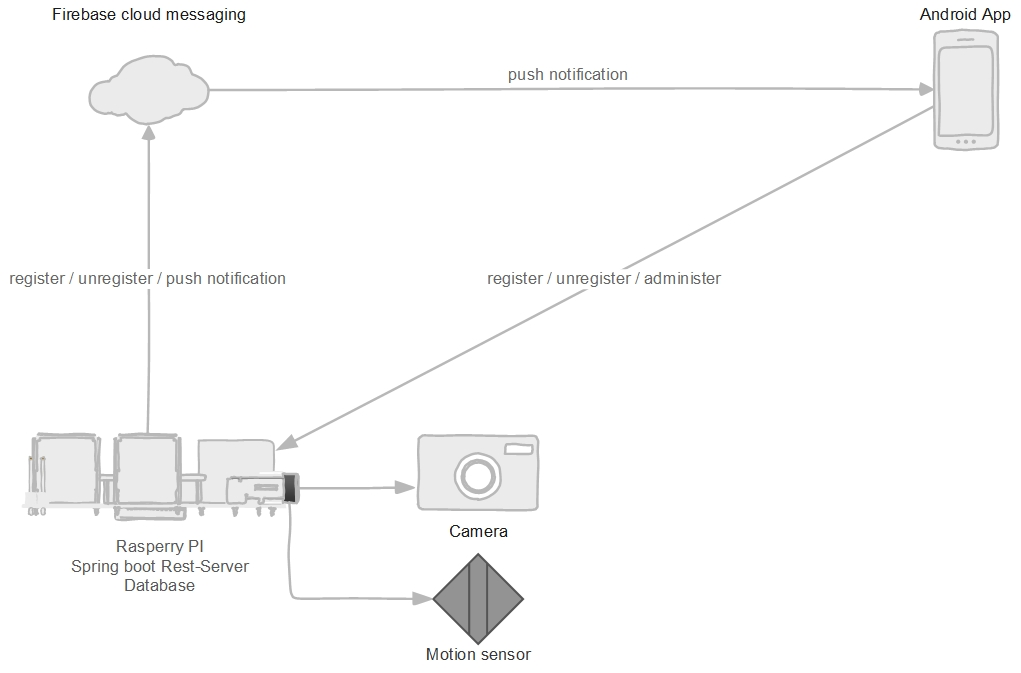
\includegraphics[scale=0.7]{\imageDir/Infrastructure.jpg}
	\caption{Systemaufbau der \emph{RPISec} Applikation}
	\label{fig:image-system-structure}
\end{figure}
\ \newpage

\subsubsection{Zugangsverifikation}
Beim Start des Systems wird vom Authentifizierungsservice \emph{(Auth-Service)} ein Administrator Benutzer erstellt, wenn dieser nicht bereits existiert. Ein neu angelegter Benutzer wird über eine E-Mail dazu aufgefordert, seinen Zugang zu aktivieren, in dem er ein Password vergibt. Im Idealfall würde die Zugangsverifikation nur im Heimnetz möglich sein.
\begin{figure}[h]
	\centering
	
\includegraphics[scale=0.5]{\imageDir/view-verify-account.JPG}
	\caption{Zugangsaktivierung}
	\label{fig:image-veriy-account}
\end{figure}
\begin{figure}[h]
	\centering
	
\includegraphics[scale=0.5]{\imageDir/view-verified-account.JPG}
	\caption{Bestätigung der Aktivierung}
	\label{fig:image-veriied-account}
\end{figure}

\subsubsection{\emph{Client Login}}
Die Abbildung \ref{fig:image-sequence-client-login} zeigt das Sequenzdiagramm, welches den Ablauf des Logins eines registrierten Benutzers über einen mobilen \emph{Client} beschreibt.
\begin{figure}[h]
	\centering
	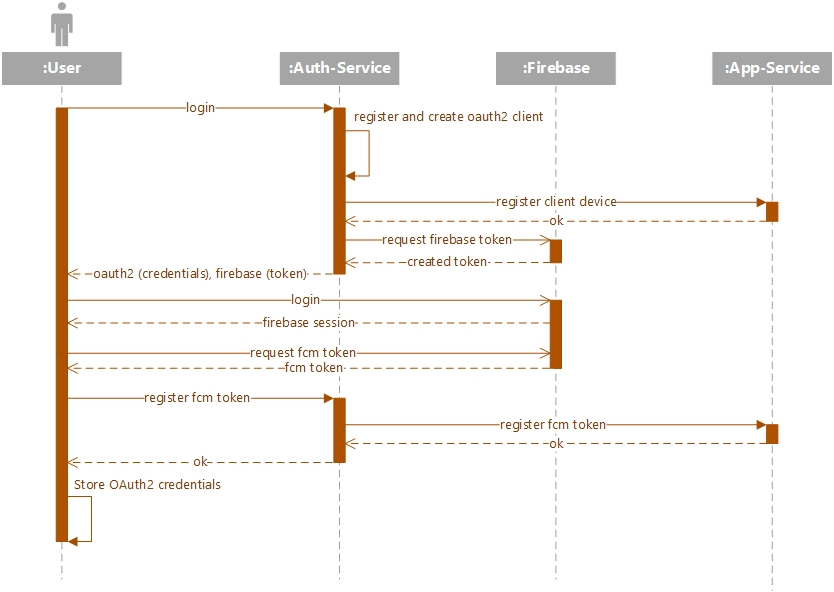
\includegraphics[scale=0.55]{\imageDir/sequence-client-login.jpg}
	\caption{Sequenzdiagramm des Benutzerlogins}
	\label{fig:image-sequence-client-login}
\end{figure}
\ \newpage
Im Zuge des Benutzerlogins wird der mobile \emph{Client} am \emph{(Auth-Service)}, der die Authentifizierung und Benutzerverwaltung verantwortlich ist und am Applikationsservice \emph{(App-Service)}, der mit der Hardware und dem \emph{Messaging} Dienst interagiert, registriert. Der \emph{Auth-Service} erstellt bei jedem Login einen neuen \emph{OAuth2-Client} und löscht gegebenenfalls einen bereits bestehenden  \emph{OAuth2-Client} für den aktuellen mobilen \emph{Client}. Das Erstellen eines \emph{OAuth2-Clients} für jeden mobilen \emph{Client} wird durchgeführt, da mit der \emph{Client}-Applikation keine \emph{Oauth2-Client} Zugangsdaten an die mobilen \emph{Clients} mit ausgeliefert werden sollen.
\newline
\newline
Dem mobilen \emph{Client} wird bei einem Login ein Authentifizierungstoken für den \emph{Cloud} Dienst übermittelt, mit dem sich der mobile \emph{Client} am \emph{Cloud} Dienst anmelden kann. Nachdem Login eines mobilen \emph{Clients} am \emph{Cloud} Dienst holt sich der mobile \emph{Client} seine eindeutige Id vom \emph{Cloud} Dienst in Form eines Tokens, der am \emph{Auth-Service} registriert wird, der wiederum den Token am \emph{App-Service} registriert, damit dieser in der Lage ist, Nachrichten an die registrierten mobilen \emph{Clients} zu versenden.  

\subsubsection{Sicherheitsverstoß melden}
\begin{figure}[h]
	\centering
	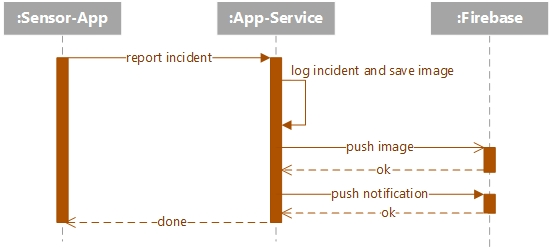
\includegraphics[scale=0.7]{\imageDir/sequence-incident.jpg}
	\caption{Sequenzdiagramm für das Behandelns eines Sicherheitsverstoßes}
	\label{fig:image-sequence-incident}
\end{figure}
\ \newline
Die Abbildung \ref{fig:image-sequence-incident} zeigt das Sequenzdiagramm für das Behandeln eines Sicherheitsverstoßes, der von der Sensorapplikation erkannt und dem Applikationsservice mitgeteilt wird. Der Sicherheitsverstoß wird über den \emph{Cloud} Dienst an die mobilen \emph{Clients} gemeldet, wobei einerseits eine Nachricht an die mobilen \emph{Clients} versendet wird, sowie das gemachte Bild in einer Onlinedatenbank den mobilen \emph{Clients} zum Download zur Verfügung gestellt wird. Die Benutzer können jederzeit auf die Onlinedatenbank zugreifen und sich die Bilder auf ihren jeweiligen mobilen \emph{Clients} herunterladen. 
\newline
\newline
Der Ansatz einen \emph{Cloud} Dienst zu verwenden sorgt dafür, dass das \emph{RPISec} System entlastet wird, da der Datenfluss und die Netzwerkzugriffe vom System ins Internet sowie umgekehrt minimiert werden. Die Daten müssen nur einmalig in die \emph{Cloud} hochgeladen werden und die Benutzer können jederzeit, beliebig oft und von jedem beliebigen mobilen \emph{Client} darauf zugreifen.
\newpage
 
\subsubsection{Nachrichtenempfang am mobilen \emph{Client}}
Die Abbildung \ref{fig:image-sequence-client-notification} zeigt den Ablauf einer Benachrichtigung eines mobilen \emph{Clients} über den \emph{Messaging} Dienst.
\begin{figure}[h]
	\centering
	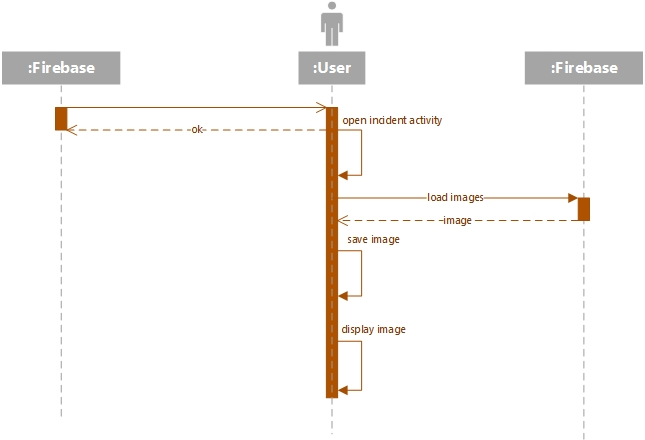
\includegraphics[scale=0.7]{\imageDir/sequence-client-notification.jpg}
	\caption{Sequenzdiagramm der Benachrichtigung eines mobilen \emph{Clients}}
	\label{fig:image-sequence-client-notification}
\end{figure}
\ \newline
Nachdem das System die mobilen \emph{Clients} via dem \emph{Messaging} Dienst über einen Sicherheitsverstoß benachrichtigt hat, erhalten die mobilen \emph{Client}-Anwendungen die Nachricht von dem \emph{Messaging} Dienst und zeigen diese an. Nachdem die Benutzer auf die Nachricht geklickt haben, wird eine \emph{Activity} für das Anzeigen der Bilder geöffnet, die alle bereits gespeicherten Bilder und das neu geladene Bild anzeigt. Diese Daten werden von der Onlinedatenbank bereitgestellt. 
\section{\emph{Raspberry PI}}
Dieser Abschnitt behandelt die verwendete Hardware für \emph{RPISec}. Für den Testaufbau wurden folgende Hardwarekomponenten verwendet.
\begin{itemize}
	\item Ein \emph{Raspberry PI 3 Model B}\footnote{\url{https://www.raspberrypi.org/products/raspberry-pi-3-model-b/}},
	\item \emph{AZDeliveryCamRasp}\footnote{\url{https://az-delivery.de/products/raspberrykamerav1-3}} und ein
	\item \emph{HC-SR501\footnote{\url{https://www.mpja.com/download/31227sc.pdf}} Bewegungssensor}.
\end{itemize}
\begin{figure}[h]
	\centering
	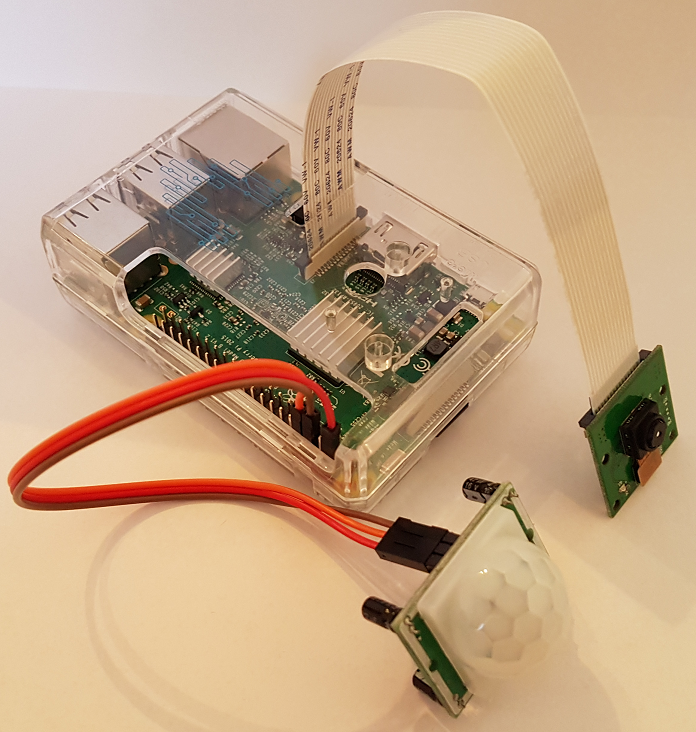
\includegraphics[scale=0.45]{\imageDir/rpisec-hardware-setup.png}
	\caption{Testaufbau der Applikation}
	\label{fig:image-hardware-setup}
\end{figure}
\ \newline
Wie in Abbildung \ref{fig:image-hardware-setup} zu ersichtlich ist, wurde die Kamera über CSI \emph{(Camera-Serial-Interface)}) und der Bewegungssensor über GPIO \emph{(General Purpose Input/Output)} an den \emph{Raspberry PI} angeschlossen.

\subsection{Betriebssysteme}
Dieser Abschnitt behandelt die verwendete Betriebssysteme für den \emph{Raspberry PI}. Die Applikation \emph{RPISec} wurde einerseits mit dem Betriebssystem \emph{hypriotos-rpi} und andererseits mit \emph{Raspian} realisiert. Das Betriebssystem \emph{hypriots} basiert auf \emph{Debian Jessie} und wird von dem \emph{OpenSource} Projekt \emph{hypriot}\footnote{\url{https://blog.hypriot.com/}} zur Verfügung gestellt wird. Das Ziel von \emph{hypriots} ist es ein Betriebssystem für \emph{Raspberry PI} zur Verfügung stellen, das bereits Docker vorinstalliert und betriebsbereit hat. Mit dem Betriebssystem \emph{Raspian} muss Docker selbst installiert, wobei Docker als Paket im \emph{Repository} zur Verfügung steht und daher sich die Installation als unkompliziert gestaltet.
\newline
\newline
Wenn Docker installiert und betriebsbereit ist, dann spielt es keine Rolle auf welchem Betriebssystem die Applikation \emph{RPISec} betrieben wird.
\newline
\newline
Da die Applikation \emph{RPISec} auf eine aktive Internetverbindung angewiesen ist, muss das Betriebssystem so konfiguriert werden, dass der \emph{Raspberry PI} entweder über \emph{Ethernet} oder \emph{Wlan} an ein Netzwerk angebunden ist, das Zugriff auf das Internet erlaubt. In einem produktiven Betrieb muss der \emph{Raspberry PI} über das Internet erreichbar sein, damit die mobilen \emph{Clients} Anfragen an die gehosteten \emph{Microservice} absetzen können.

\section{Software}
Dieser Abschnitt behandelt die verwendete bzw. implementierte Software für \emph{RPISec}.
\subsection{\emph{Microservices} und \emph{Cloud}}
Dieser Abschnitt behandelt die auf dem \emph{Raspberry PI} gehosteten Services. Die Services wurden mit \emph{Spring Boot} als \emph{Microservices} implementiert, was möglich war, da Oracle eine ARM Implementierung der Java-JDK bereitstellt und die \emph{Microservices} schlank implementiert wurden, sodass die zur Verfügung stehenden Ressourcen ausreichen, um diese Services auf einen \emph{Raspberry PI} zu betreiben.
\newline
\newline
Es wurden die beiden \emph{Microservices} \emph{rpisec-auth-service} für die Benutzerverwaltung und OAuth2 Authentifizierung und \emph{rpisec-app-service} für die Interaktion mit der Sensorik und der Interaktion mit dem \emph{Cloud}-Diensten implementiert, wobei der \emph{Microservice} \emph{rpisec-auth-service} im Zuge des Projekts für die Lehrveranstaltung \emph{Service Engineering} implementiert wurde. Es hätte auch ausgereicht die Benutzerverwaltung in den \emph{Microservice rpisec-app-service} zu verpacken, obwohl dann der \emph{Microservice} für zwei Aspekte verantwortlich gewesen wäre was im Widerspruch zu einem \emph{Microservice} steht, der nur für einen Aspekt verantwortlich sein soll. 
\newline
\newline
Der Microservice \emph{rpisec-app-service} interagiert nicht direkt mit der Sensorik, sondern bindet die Sensorapplikation beschrieben in Abschnitt \ref{sec:sensor-application} ein und ist für dessen Lebenszyklus verantwortlich. Nachdem Start der Sensorapplikation wird ein \emph{Listener} registriert, der auf Statusänderungen des Bewegungssensor reagiert und diesen Sicherheitsvorfall wie in Abbildung \ref{fig:image-sequence-incident} behandelt.
\newline
\newline
Die beiden \emph{Microservices} müssen Daten persistent halten und sind daher auf eine Datenbank angewiesen, wobei im Entwicklungsbetrieb auf einen Entwicklerrechner H2 und im produktiven Betrieb auf einen \emph{Raspberry PI} PostgreSQL verwendet wird. Die Datenbank PostgreSQL konnte verwendet werden, da PostgreSQL die ARM Architektur unterstützt.
\newline
\newline
Als \emph{Cloud} Anbieter wurde \emph{Google} gewählt, welcher die Plattform \emph{Firebase} anbietet, die eine JSON-Datenbank und einen \emph{Cloud Messaging} Dienst anbietet. Für diesen Dienst gibt es eine Java Implementierung das sogenannte \emph{firebase-admin-sdk}, das eine API zum Interagieren mit der JSON-Datenbank und eine API zum Erstellen von Authentifizierungstoken für die \emph{Client}-Authentifizierung bei Firebase zur Verfügung stellt. In der Java Implementierung wird zurzeit keine API für die Interaktion mit dem \emph{Messaging} Dienst zur Verfügung gestellt, was aber kein Problem darstellt, da es sich hierbei um eine einfache Anfrage an eine \emph{REST-API} handelt, die mit Spring \emph{RestTemplate} durchgeführt wird.
\section{\emph{Docker} Infrastruktur}
Dieser Abschnitt behandelt die \emph{Docker} Infrastruktur, welche die Service und deren Abhängigkeiten \emph{hosted}. Da der Umgang mit Docker und einer umfangreicheren Infrastruktur mit viel Shell-Skripten verbunden ist, wird das Python basierte Tool \emph{Docker-Compose} verwendet, das es erlaubt eine Infrastruktur, die aus einer Menge von untereinander abhängigen Services besteht, deklarativ über eine \emph{YAML}-Konfigurationsdatei zu konfigurieren. 
\newline
\newline
Die Definition der \emph{Images} sowie der Aufbau der \emph{Docker} Infrastruktur sind im Verzeichnis \emph{$/host/docker/$} enthalten, wobei die einzelnen \emph{Dockerfiles} der Services in Unterverzeichnissen organisiert, die alle Abhängigkeiten, welche in die Images mitaufgenommen werden, enthalten. Die \emph{PostgreSQL} Images stehen am \emph{Docker Hub}\footnote{https://hub.docker.com/r/tobi312/rpi-postgresql/} zur Verfügung.   
\begin{center}
	\begin{figure}[h]
		\centering
		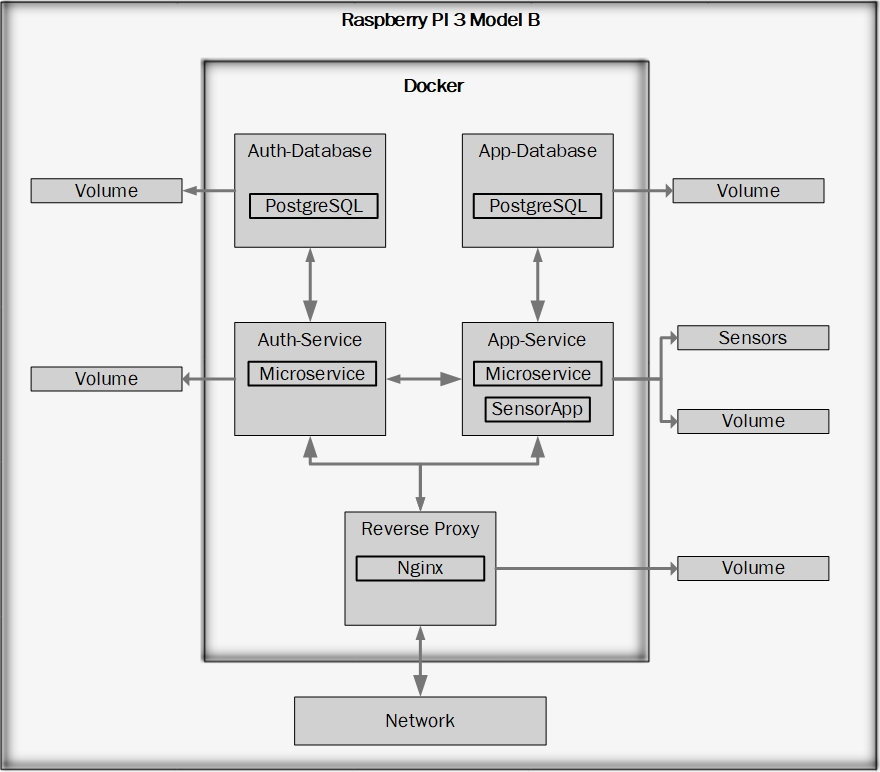
\includegraphics[scale=0.7]{\imageDir/pi-docker-infrastructure.jpg}
		\caption{\emph{Raspberry PI Docker} Infrastruktur}
		\label{fig:rapsi-docker-infrastructure}
	\end{figure}
\end{center}
Die Abbildung \ref{fig:rapsi-docker-infrastructure} zeigt die \emph{Docker} Infrastruktur, wie sie am \emph{Raspberry PI} angewendet wird. Da die Daten persistent gehalten werden müssen, werden die Daten in den \emph{Containern} in Verzeichnissen gehalten, die auf den \emph{Host} über ein \emph{Volume} gebunden sind. Der \emph{Docker Container App-Service} benötigt privilegierte Rechte damit die Sensorapplikation mit der angeschlossenen \emph{Hardware} kommunizieren kann. Die benötigten C-Bibliotheken wie \emph{WiringPI}\footnote{https://git.drogon.net/?p=wiringPi;a=summary} und die Bibliotheken für das Interagieren mit der \emph{Raspberry Pi GPU}\footnote{https://github.com/raspberrypi/userland} werden in einem Basisimage während des Bauens geladen und kompiliert. Dieses Basisimage stellt die Basis aller eigenen Images dar.
\begin{code}
	\caption{docker-compose.yml für RPISec am \emph{Raspberry PI}}
	\yamlFile{\dockerRPIDir/docker-compose.yml}
	\label{src:test-docker-compose}
\end{code}
Der Quelltext \ref{src:test-docker-compose} zeigt den Inhalt der \emph{docker-compose.yml}, welche die \emph{Docker} Infrastruktur für \emph{RPISec} am \emph{Raspberry PI} definiert. Die in der Datei vorkommenden Textfragmente im Format \emph{\$\{...\}} stellen Variablen dar, die \emph{Docker-Compose} entweder aus einer Datei mit dem Namen \emph{.env}, die auf derselben Ebene wie die \emph{docker-compose.yml} platziert werden muss, oder aus den Umgebungsvariablen des Benutzers, mit dem die Infrastruktur erstellt wird, auflöst. Sollten Variablen nicht auflösbar sein, so wird eine entsprechende Meldung auf die Konsole ausgegeben.
\newline
\newline
Das Bauen der Infrastruktur und Starten der Services dauert am \emph{Raspberry PI} relativ lange, da nur wenig Speicher zur Verfügung steht, es sich um eine ARM-Architektur handelt und das Speichermedium eine \emph{MicroSD} Karte ist. Ebenso ist die Performance der Services nicht herausragend, jedoch kann die Applikation auf dem \emph{Raspberry PI} problemlos ausgeführt werden.  
\section{Erfahrungen}
Dieser Abschnitt behandelt die gemachten Erfahrungen während der Umsetzung dieses Projekts. Nachdem für dem \emph{Raspberry PI} bereits ein Betriebssystem zur Verfügung steht, das alle benötigten Bibliotheken für wie \emph{Docker} und \emph{Docker-Compose} bereitstellt und es auch eine \emph{ARM} Implementierung von \emph{Oracle}-Java gibt, hat sich die Umsetzung als relativ einfach gestaltet. Hätte es keine Oracle Implementierung für die \emph{ARM}-Plattform gegeben, hätte man \emph{OpenJDK} verwenden müssen, was das Laufzeitverhalten der \emph{Microservices} negativ beeinflusst hätte.   
\newline
\newline
Die verwendete \emph{PostgreSQL} Datenbank, die in einem \emph{Docker Container} gehostet wird, braucht beim ersten Start (Keine Datenbank vorhanden) relativ lange, weswegen der erste Start der \emph{Docker-Compose} orchestrierten  Infrastruktur beim ersten Mal fehlschlägt, da die \emph{Microservices} gestartet sind und auf eine nicht verfügbare Datenbank zugreifen wollen, die noch im Initialisierungsprozess feststeckt. Dieses Problem wurde gelöst indem die Datenbanken initialisiert werden, bevor die gesamte Infrastruktur gestartet wird.
\newline
\newline
Die Java Bibliothek für den \emph{Cloud}-Dienst \emph{Firebase} ist zwar eingeschränkt verglichen mit der Implementierung für \emph{NodeJS}, jedoch konnten alle Tasks, bis auf das Versenden der \emph{Messages}, das mit Spring \emph{Resttemplate} realisiert wurde, einfach implementiert werden. 
\newline
\newline
Für die Umsetzung der \emph{Microservices} mussten keine besonderen Vorkehrungen wegen dem Hosten auf einen \emph{Raspberry PI} getroffen werden. Nichts desto trotz sollte man sich bei der Implementierung der \emph{Microservices} bezüglich der Abhängigkeiten und verwendeten \emph{Frameworks} bewusst sein, dass man mit einem System konfrontiert ist, das nur beschränkte Ressourcen zur Verfügung stellt.
\newline
\newline
Abschließend kann man sagen das \emph{Docker} und Java Programme auf einen \emph{Raspberry PI} sehr gut zu betreiben sind, solange man nicht Programme und \emph{Docker Container} betreiben will, für welche die zur Verfügung stehenden Ressourcen nicht oder nur knapp ausreichen. Vor allem das Zeitverhalten muss berücksichtigt werden, dass aufgrund der \emph{ARM}-Architektur sich nicht gleich verhält als auf einer \emph{x86}-Architektur. \emph{PI4J} bietet einen sehr gute \emph{API} für die Interaktion mit den \emph{GPIO} und für das Ausführen von Prozessen am Hostsystem.  


% Quellen
% AZDeliveryPICam:
% https://www.amazon.de/dp/B01M6UCEM5/ref=pe_386171_51767411_TE_dp_3
% -------------------------------------------------------------------
% HC-SR501
% https://www.amazon.de/dp/B00TI2ZC72/ref=pe_386171_38075861_TE_item
% -------------------------------------------------------------------
% HC-SR501 Schema
% ttp://www.netzmafia.de/skripten/hardware/RasPi/Projekt-PIR/
% -------------------------------------------------------------------

\end{document}          
